
% !TEX root = ../main.tex

% Local Variables:
% TeX-master: "../main"
% End:
% chktex-file 26

%%%%%%%%%%%%%%%%%%%%%%%%%%%%%%% Header %%%%%%%%%%%%%%%%%%%%%%%%%%%%%%%%%%%%%%%%%%%%
\begin{minipage}[l]{0.42\textwidth}
    \includegraphics[width=1\textwidth]{img/logo-UNAMBA.png}
\end{minipage}
\hfill
\begin{minipage}[c]{0.5\textwidth}
    \begin{flushright}
	\large{\textbf{Unidad \#1}}\\
	\large{Lectures on Física III}\\
	\large{06 de octubre del 2025. Haquira, Apurimac}\\
        % \large{\textbf{Student:} Huallpa Aimituma Josué David}
    \end{flushright}
\end{minipage}
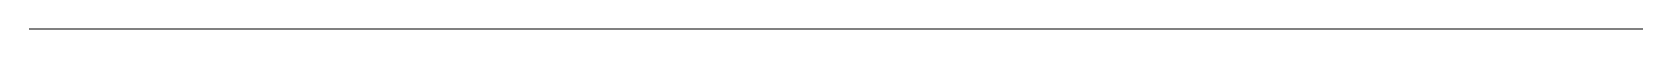
\begin{tikzpicture}
    \draw[gray,thick] (-6.5,0)--(14,0);
\end{tikzpicture}


 %%%%%%%%%%%%%%%%%%%%%%%% INICIO DEL CONTENIDO EN DOS COLUMNAS %%%%%%%%%%%%%%%%%%%%%
  
 \begin{multicols}{2}
   \begin{center}
         \LARGE{\textbf{Capítulo I: Electrostática}}\\	
         \vspace{0.2cm}
         % \Large {Lecturers Esteban Chalbaud \& Daniel Galviz} \\
         % \large{Teaching Assistant: Mauricio Gamonal \& Irvin Martínez}\\
         % \large{PhysicsLatam.com}\\
         % \vspace{0.2cm}
         \large{24 Septiembre 2025, 6:59 am (GMT-4)}\\
         % \vspace{0.2cm}
         \large{— Ficha de Trabajo —}
     \end{center}
\section{coordenadas cilindricas}
Un sistema de coordenadas cilíndricas es útil pa
ra resolver problemas que tienen simetría cilíndri
ca, como calcular la capacitancia por unidad de
 longitud de una línea de transmisión coaxial.
 \begin{equation}
    \vec{A}\times \vec{B} = \begin{vmatrix}
\vec{\imath} & \vec{\jmath}  & \vec{k} \\
A_x & A_y & A_z\\
5 & 0 & 3
\end{vmatrix}
 \end{equation}


\end{multicols}
